\subsection{The Inverse CDF technique}

\begin{frame}{Inverse cumulative distribution function (CDF)}

\only<1,2>{
\begin{center}
\begin{minipage}{0.45\textwidth}
	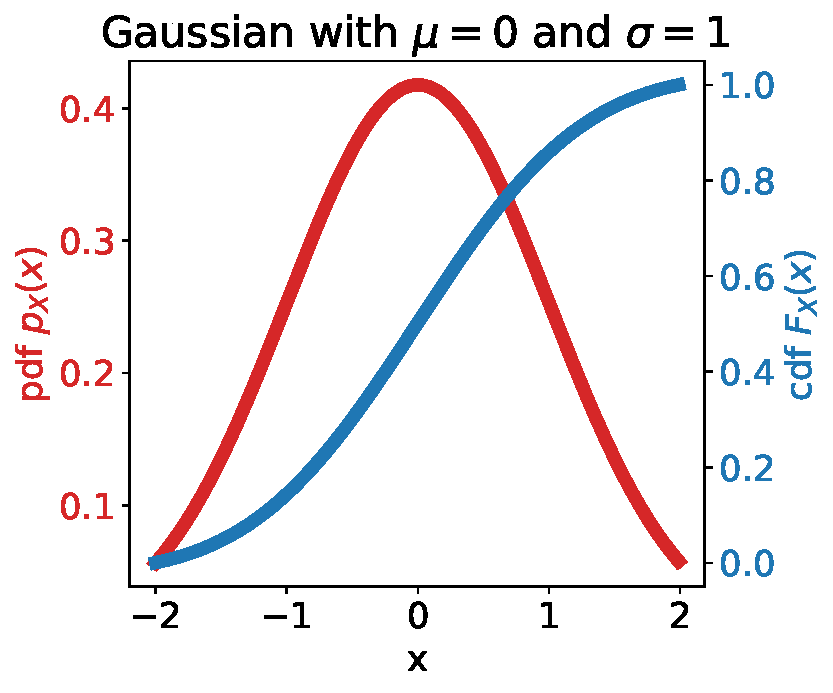
\includegraphics[width=0.99\textwidth]{img/gauss_pdfcdf}
\end{minipage}
\begin{minipage}{0.45\textwidth}
	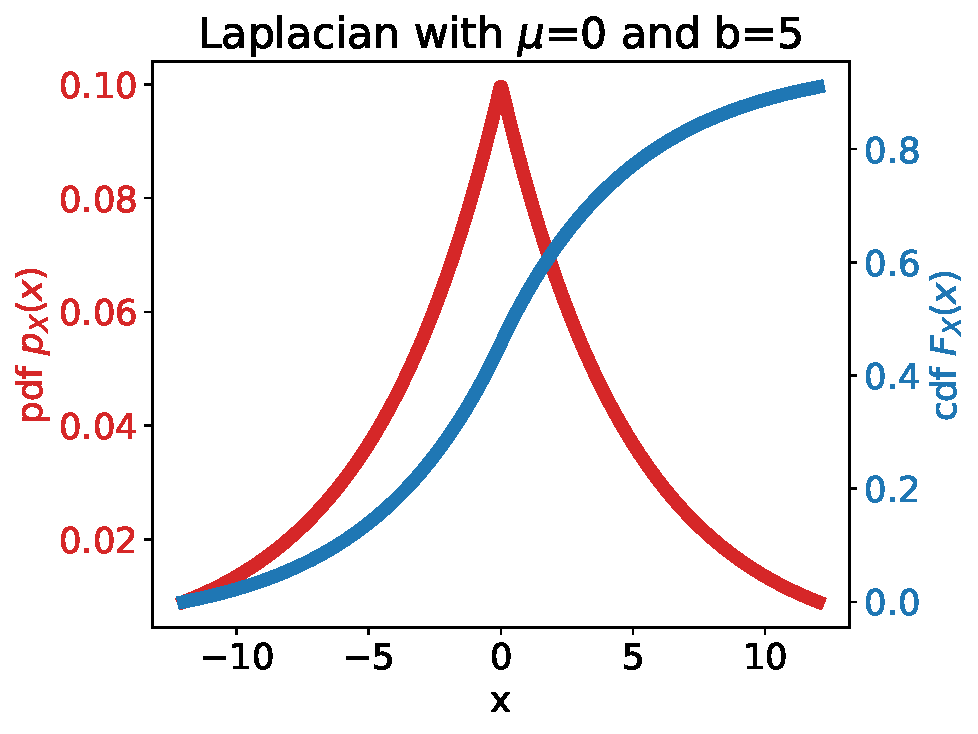
\includegraphics[width=0.99\textwidth]{img/laplacian_pdfcdf}
\end{minipage}
\end{center}
}
\pause

If $F_{X}(x)$ is the cumulative
  distribution function (cdf) of a random variable $X$, then the
random variable $Z = F_{X}(X)$ is uniformly distributed on the
interval $[0,1]$. 

\only<3>{
\begin{center}
\begin{minipage}{0.45\textwidth}
	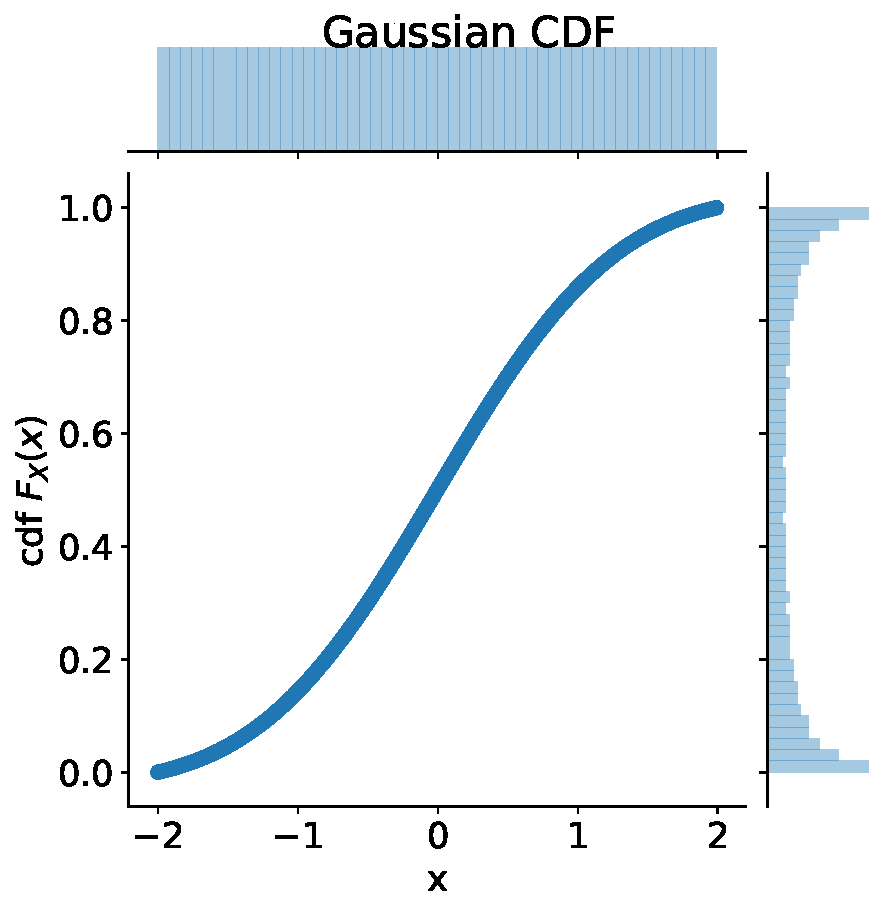
\includegraphics[width=0.99\textwidth]{img/gauss_cdfmarginals}
\end{minipage}
\begin{minipage}{0.45\textwidth}
	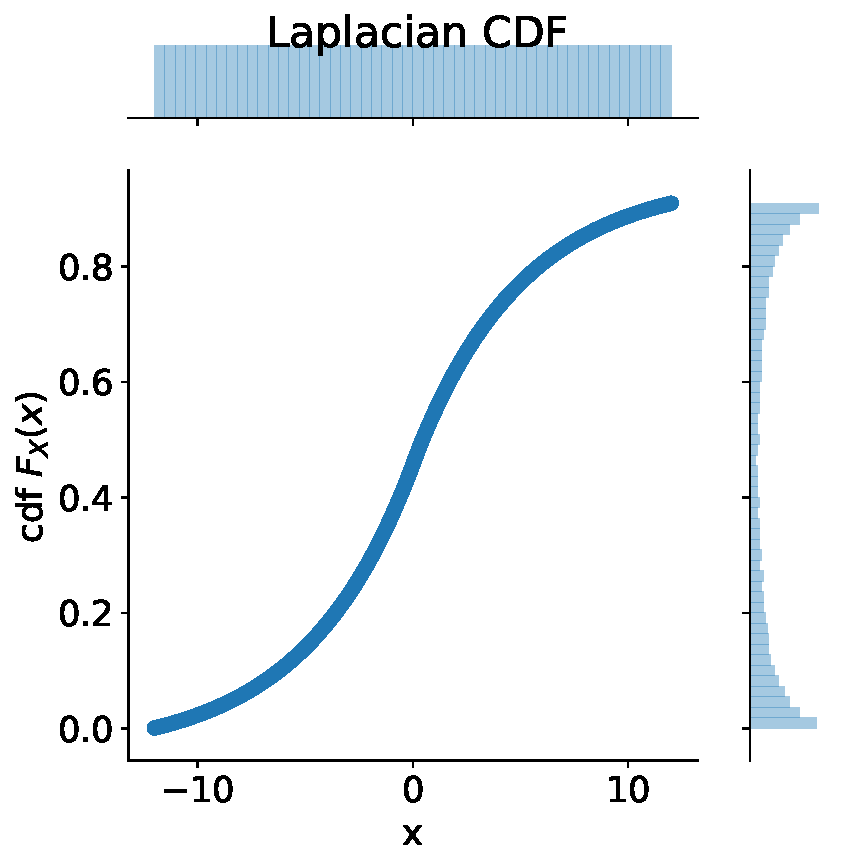
\includegraphics[width=0.99\textwidth]{img/laplacian_cdfmarginals}
\end{minipage}
\end{center}
}

\end{frame}

\begin{frame}


This result provides 
% (after inverting the relationship) 
a general recipe to generate
samples $\tilde x$ of a random variable $X$ with a desired pdf $p_X(x)$
from uniformly distributed random numbers $\tilde z \in [0,1]$:
\begin{enumerate}
\item Compute the cdf $F_X(x)$ of the desired pdf $p_X(x)$

\begin{equation}
F_X(x) = P(X \leq x) = \int_{-\infty}^{x} p(y)\,dy
\end{equation}

The cdf is a one-to-one (bijective) mapping of the domain of the cdf to the interval $[0,1]$.
 If $Z$ is a uniform random variable, then $X=F_X^{-1}(Z)$ has the distribution $F$.

\item Determine the inverse transformation $F^{-1}$.

\item Sample uniformly distributed numbers (in $[0,1]$), $\tilde z$.
\item Get the samples $\tilde x=F^{-1}(\tilde z)$ from $X$. 
\end{enumerate}

At this point we can use a PRNG to sample from the uniform distribution and 
by plugging those samples into the inverse cdf we can obtain samples from a desired pdf.


\end{frame}

\begin{frame}

Note that this relies on \textbf{having the cdf} to get its inverse. We might not have this information.

\pause

\slidesonly{
\begin{center}
	
\includegraphics[width=0.4\textwidth]{img/meme_gobigger}
\end{center}
}

\end{frame}
